\chapter{Visualization}

\begin{figure}[h]
  \centering
  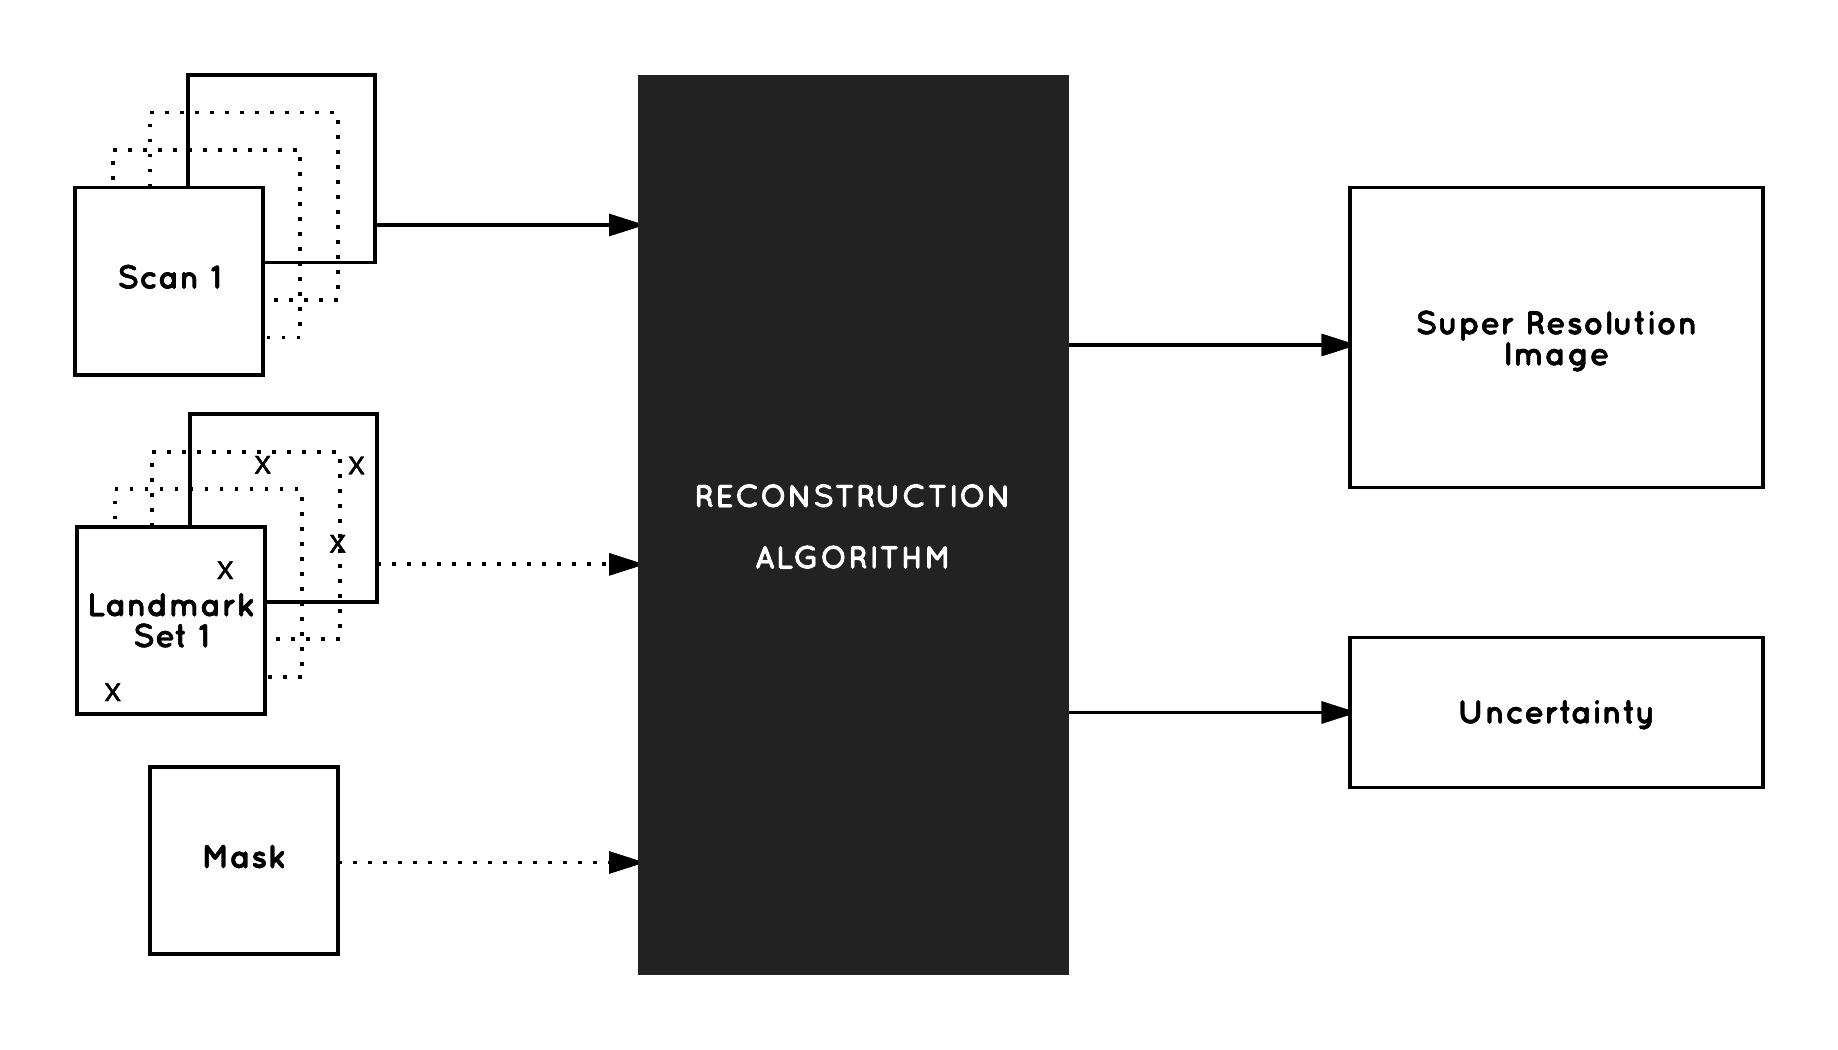
\includegraphics[width=0.8\textwidth]{images/reconstruction_overview.png}
  \caption{Reconstruction Overview}
  \label{fig:erosionbefore}
\end{figure}

The super resolution reconstruction process takes in a set of slice stacks (scans), an optional mask and outputs the reconstructed MRI volume and the uncertainty. The mask is used to ignore areas that are not of interest; for example when doing a fetal scan a mask can be created to ignore surrounding areas like the womb and amniotic fluid.

\section{Preprocessing}\label{section:preprocessing}
The uncertainty tells us for each pixel in the reconstructed volume how much confidence we have in that value. However, before we can visualize it some preprocessing must be applied. 

\subsection{Normalization}
The uncertainty is linearly scaled so each value is between 0 and 1.

\begin{verbatim}
  0 - no information (high uncertainty - worst)
  1 - maximum information (low uncertainty - best)
\end{verbatim}

\subsection{Erosion}
The optional erosion step removes the uncertainty values at the edge of the reconstruction. The edges often have a much higher uncertainty either because there are fewer slices to use or the mask cuts off the data required. Removing this edge helps the visualization to focus on the core of the volume.

The edges are removed in five steps:

\begin{enumerate}
  \item An erosion filter is applied to the image. This removes the edges but has the unwanted effect of also eroding uncertainty in the center of the volume.
  \item The absolute difference is taken between the original and the eroded image.
  \item The difference is then thresholded to create a mask of the areas that changed the most. The idea here is that the edges change significantly more than the small pockets of uncertainty inside.
  \item A growing filter is applied to the mask, to ensure the entire edge is covered.
  \item Finally all the points in the mask are set to 0 to remove the edge.
\end{enumerate}

Figure \ref{fig:erosionoverview} shows how the soft fade out of uncertainty due to the mask is removed to create a hard edge.

\begin{figure}[h]
  \centering
  \begin{subfigure}[b]{0.3\textwidth}
    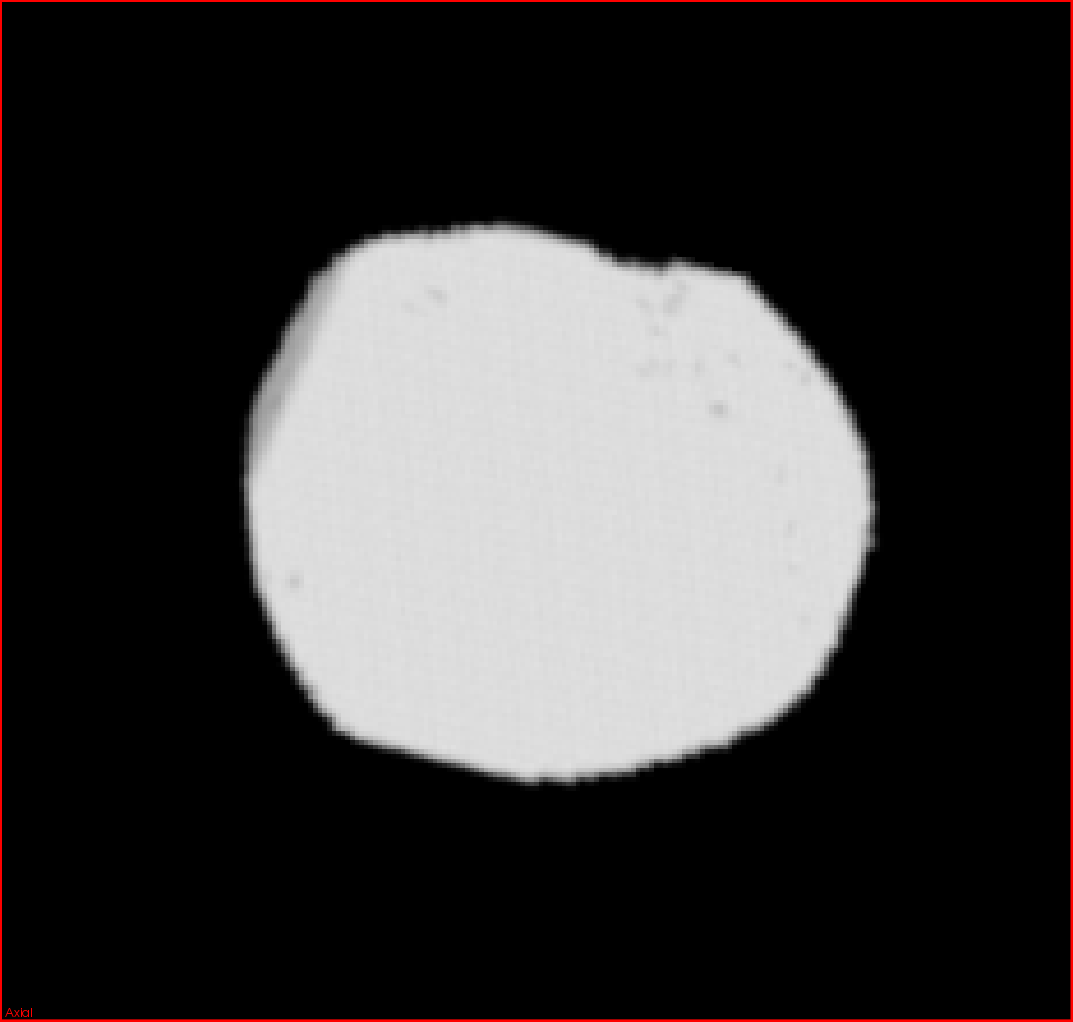
\includegraphics[width=\textwidth]{images/erosion_0.png}
    \caption{Original}
    \label{fig:erosion0}
  \end{subfigure}%
  ~ %add desired spacing between images, e. g. ~, \quad, \qquad, \hfill etc.
    %(or a blank line to force the subfigure onto a new line)
  \begin{subfigure}[b]{0.3\textwidth}
    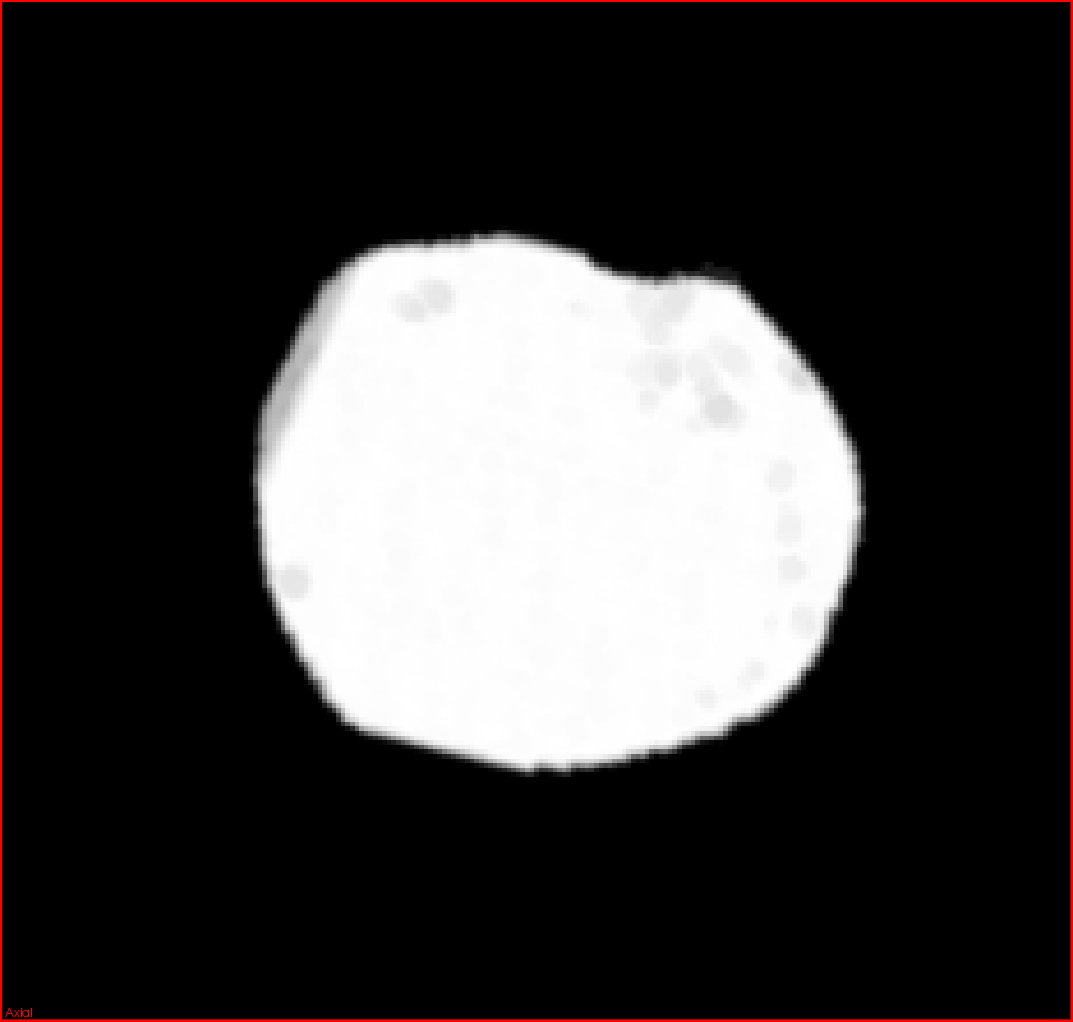
\includegraphics[width=\textwidth]{images/erosion_1.png}
    \caption{Step 1}
    \label{fig:erosion1}
  \end{subfigure}  
  ~ %add desired spacing between images, e. g. ~, \quad, \qquad, \hfill etc.
    %(or a blank line to force the subfigure onto a new line)
  \begin{subfigure}[b]{0.3\textwidth}
    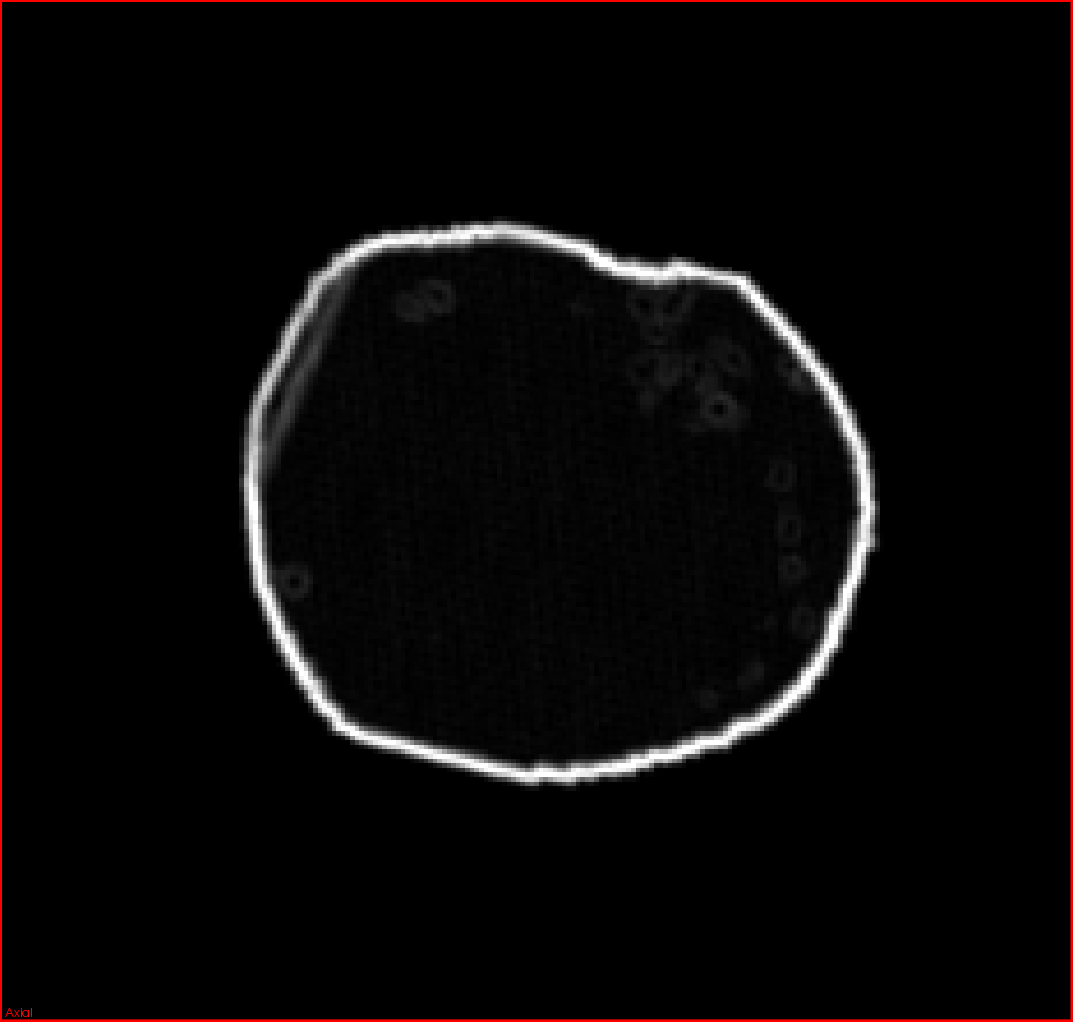
\includegraphics[width=\textwidth]{images/erosion_2.png}
    \caption{Step 2}
    \label{fig:erosion2}
  \end{subfigure}
  ~ %add desired spacing between images, e. g. ~, \quad, \qquad, \hfill etc.
    %(or a blank line to force the subfigure onto a new line)
  \begin{subfigure}[b]{0.3\textwidth}
    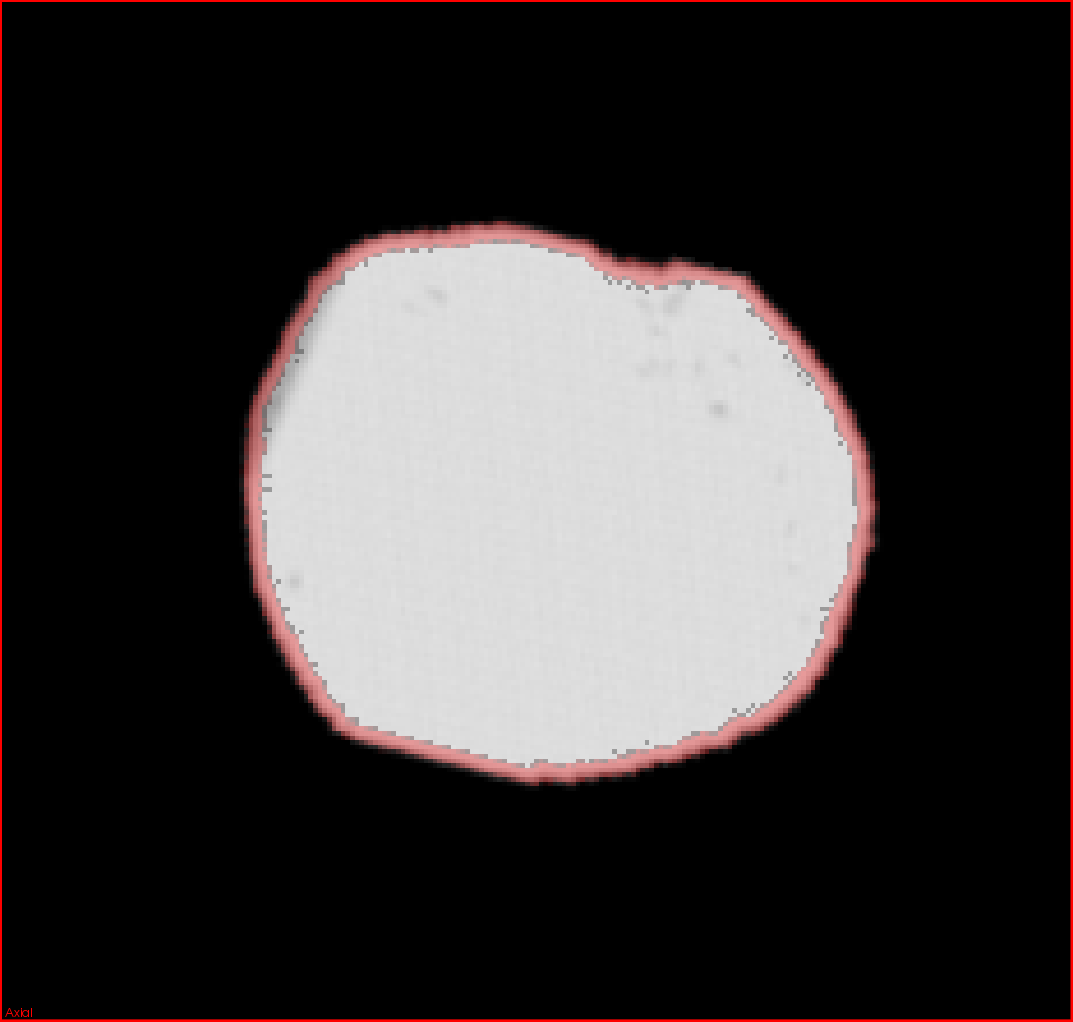
\includegraphics[width=\textwidth]{images/erosion_3.png}
    \caption{Step 3}
    \label{fig:erosion3}
  \end{subfigure}%
  ~ %add desired spacing between images, e. g. ~, \quad, \qquad, \hfill etc.
    %(or a blank line to force the subfigure onto a new line)
  \begin{subfigure}[b]{0.3\textwidth}
    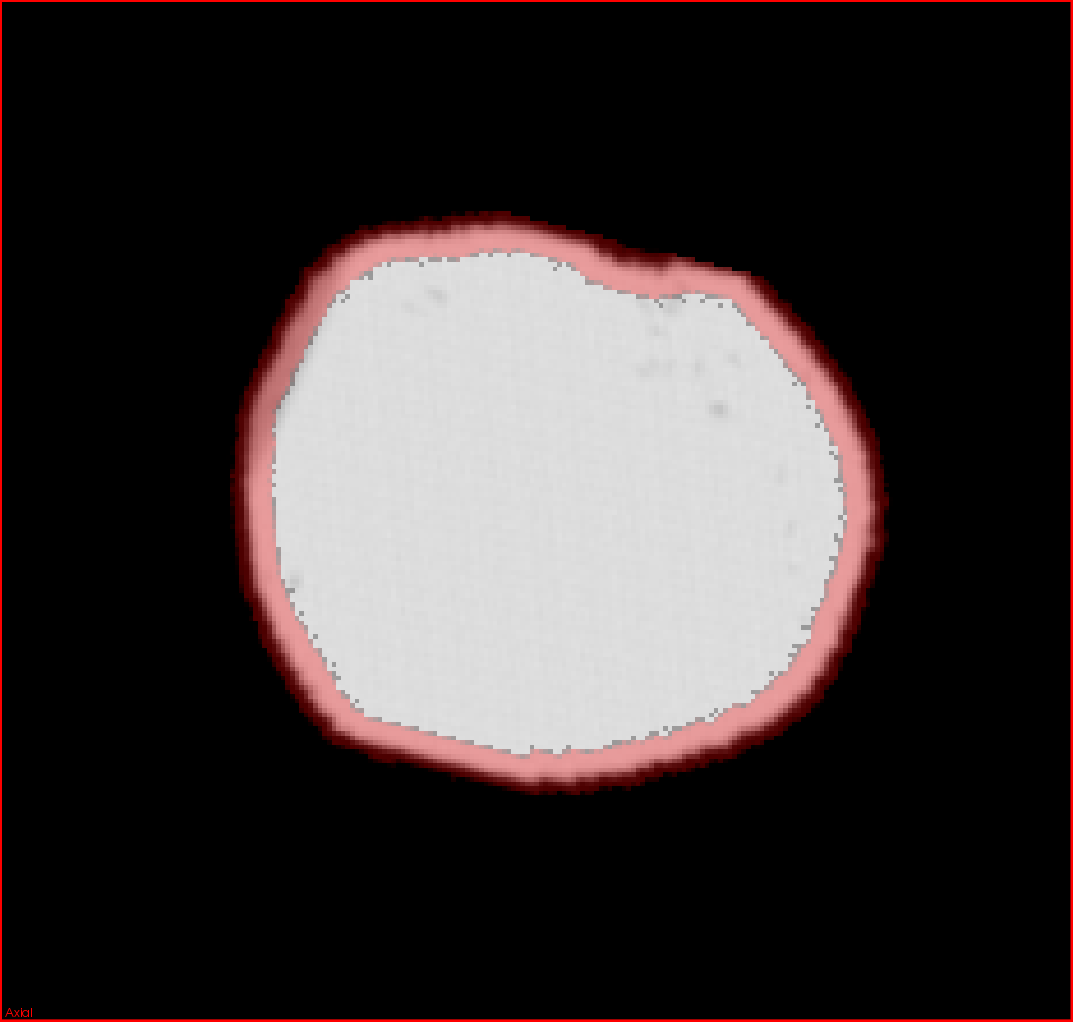
\includegraphics[width=\textwidth]{images/erosion_4.png}
    \caption{Step 4}
    \label{fig:erosion4}
  \end{subfigure}  
  ~ %add desired spacing between images, e. g. ~, \quad, \qquad, \hfill etc.
    %(or a blank line to force the subfigure onto a new line)
  \begin{subfigure}[b]{0.3\textwidth}
    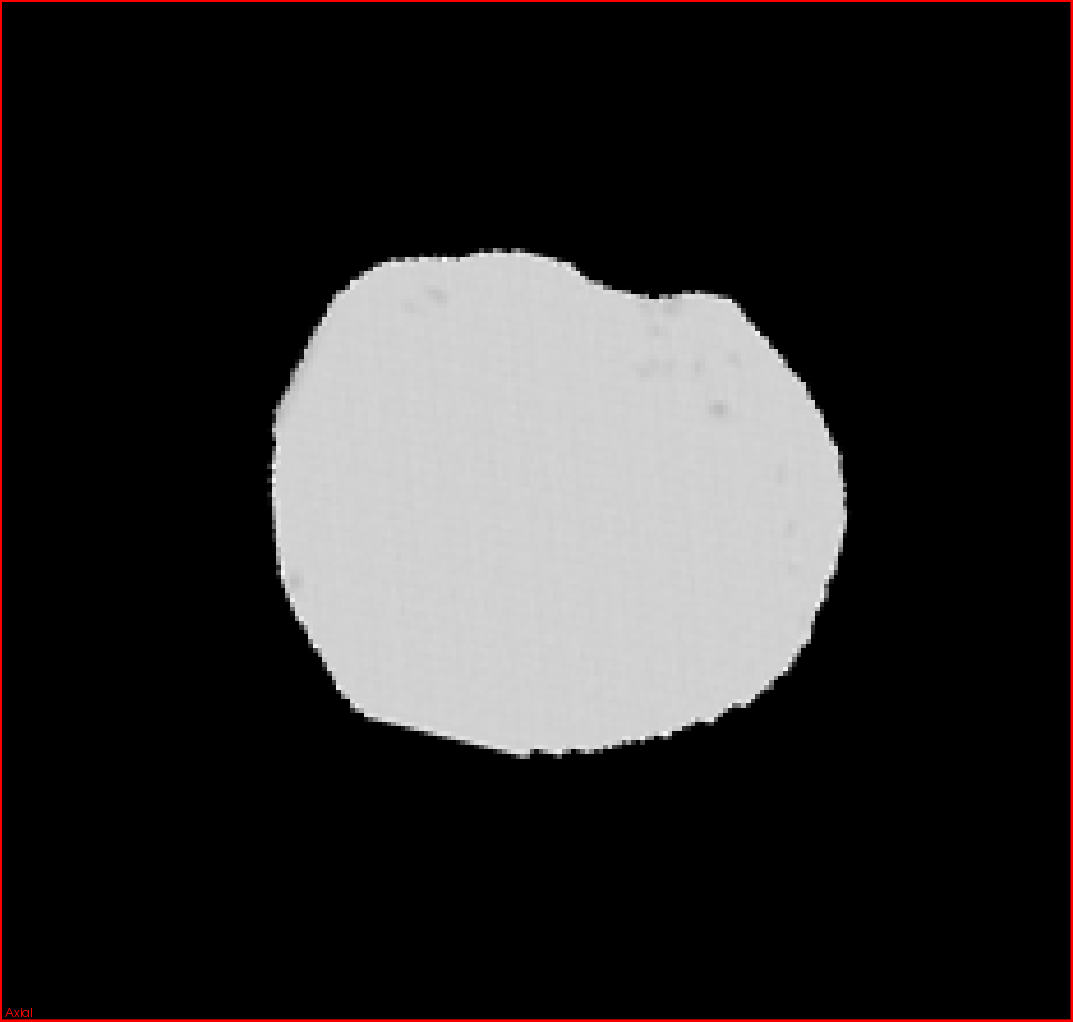
\includegraphics[width=\textwidth]{images/erosion_5.png}
    \caption{Step 5}
    \label{fig:erosion5}
  \end{subfigure}  
  \caption{Steps involved in removing the edge.}\label{fig:erosionoverview}
\end{figure}

% Idea -> Implementation -> Results
\newpage
\section{Thresholding}\label{section:thresholding}

The idea behind thresholding is to isolate areas in the reconstructed image within a particular range of uncertainty. This allows the viewer to highlight regions in a specified range (e.g. 0.2 to 0.5) and also lets them isolate the worst values in the volume (e.g. the worst 1$\%$).

\subsection*{Implementation}
The implementation uses a filter provided by ITK to go create a binary mask which is set to 1 where the uncertainty is in the range and 0 where it is not. This mask is then overlayed on the reconstructed scan in 2D and made transparent so both the uncertain area and underlying scan can be seen simultaneously.

Two variations on the volume rendering approach have been implemented to view the threshold in 3D.

Variation 1 - Volume Render the Uncertainty:
<graph> Transfer Function (transparency): (0, 0), (min - epsilon, 0), (min, 1), (max, 1), (max + epsilon, 0), (1, 0)

The problem that was found with variation 1 was that the renderer draws the edge of the uncertainty, even though it had previously been removed by erosion. This is due to the renderer using linear interpolation to take samples along each ray fired into the volume. Figure <SOMETHING> illustrates the problem - the background has value 0.0, and the start of the uncertainty has a value of approximately ~0.6. This means that points interpolated between the two get values in the range 0.0-0.6, for example 0.3, when there is only uncertainty 0.0 and 0.6 there.

Variation 2 - Volume Render the Mask:
<graph> Transfer Function (transparency): (0, transparent), (1, opaque)

This thresholded mask is also displayed in 3D using volume rendering (see section \ref{background:volumerendering}). The transfer function used maps a value of 0 (out of the range) to be completely transparent and a value of 1 (in the range) to be opaque.

\begin{figure}[h]
  \centering
  \begin{subfigure}[b]{0.5\textwidth}
    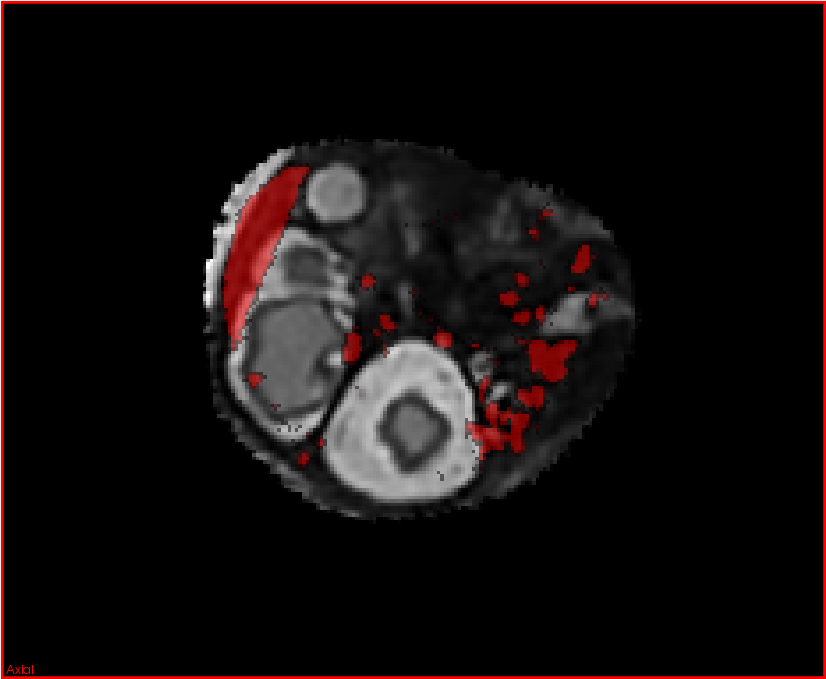
\includegraphics[width=\textwidth]{images/thresholding_2d.png}
    \caption{2D Thresholding}
    \label{fig:thresholding2d}
  \end{subfigure}%
  ~ %add desired spacing between images, e. g. ~, \quad, \qquad, \hfill etc.
    %(or a blank line to force the subfigure onto a new line)
  \begin{subfigure}[b]{0.5\textwidth}
    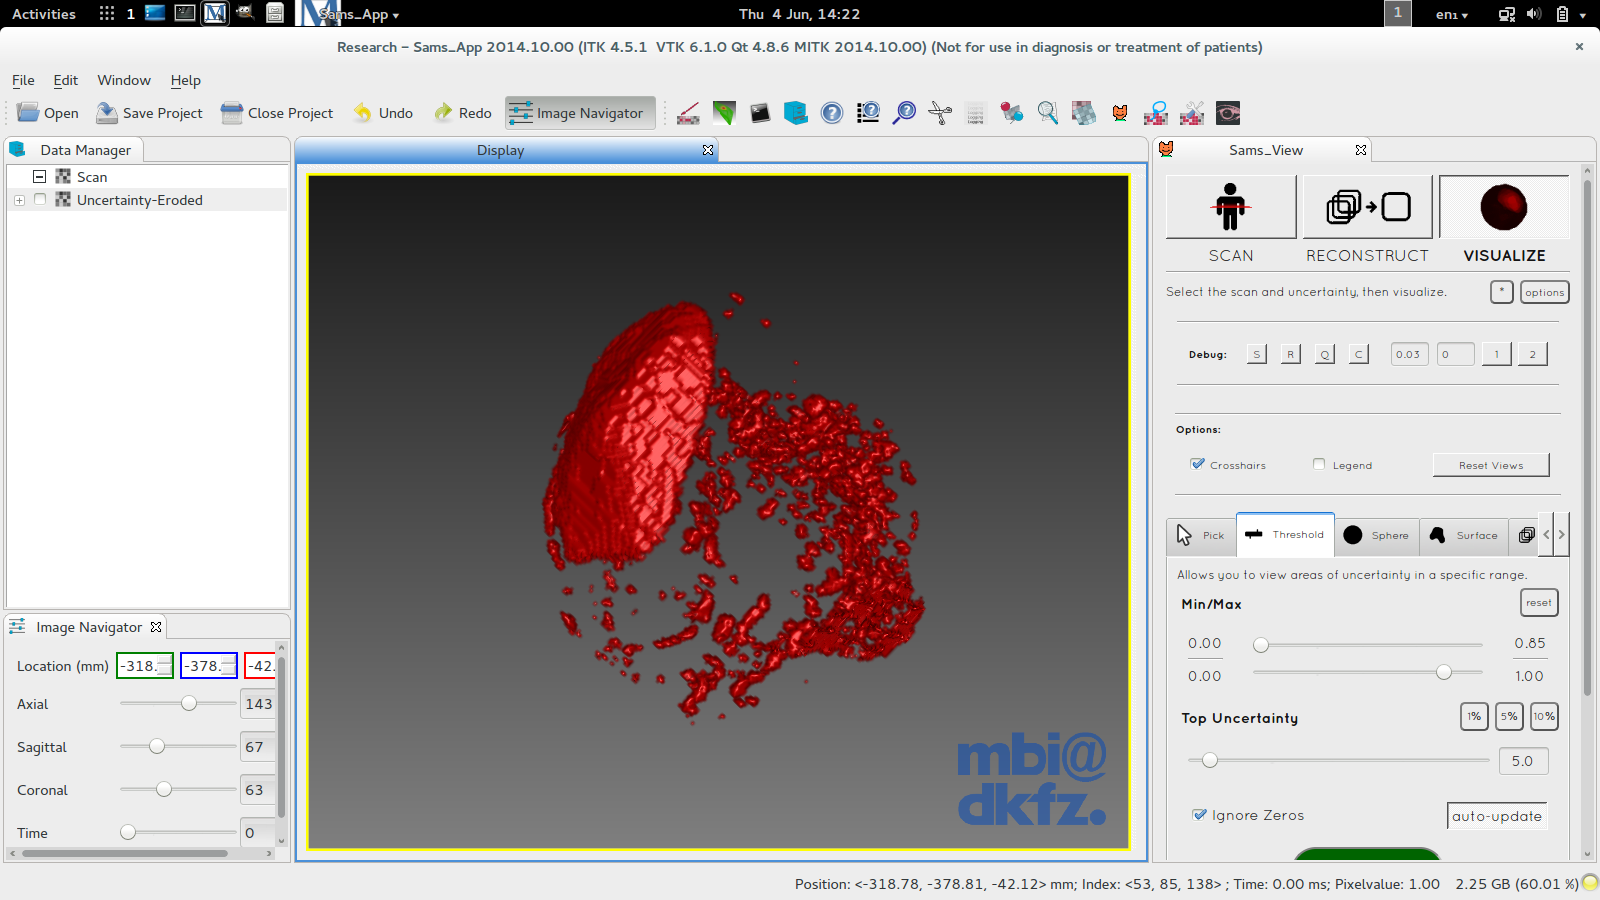
\includegraphics[width=\textwidth]{images/thresholding_3d.png}
    \caption{3D Thresholding}
    \label{fig:thresholding3d}
  \end{subfigure}
  \caption{Example showing the worst 5$\%$ of an example reconstruction.}\label{fig:threshldingoverview}
\end{figure}

\subsection*{Results}
// Compare with applying transfer function to actual uncertainty. Illustrate the problems with small dots.

\newpage
\section{Uncertainty Surface}\label{section:uncertaintysurface}

\newpage
\section{Next Scan Plane}\label{section:nextscanplane}

\newpage
\chapter{Tool}

\newpage
\section{Scan Simulation}\label{section:simulatescan}

\newpage
\section{Reconstruction}\label{section:reconstruction}